\documentclass[12pt]{ucthesis}

\usepackage{etex}
\usepackage[morefloats=125]{morefloats}
\usepackage[hyphens]{url}
\usepackage{subfig}
\usepackage{graphicx}
\usepackage{tabularx}
\usepackage{amssymb}
\usepackage{amsmath}
\usepackage[letterpaper]{geometry}
\usepackage[overload]{textcase}
\usepackage[nonumberlist,toc]{glossaries}
\usepackage{wrapfig}
\usepackage{longtable}
\usepackage{morefloats}
\usepackage{float}
\usepackage{listings}
\usepackage{color}
\usepackage{colortbl}
 
\definecolor{codegreen}{rgb}{0,0.6,0}
\definecolor{codegray}{rgb}{0.5,0.5,0.5}
\definecolor{codepurple}{rgb}{0.58,0,0.82}
\definecolor{backcolour}{rgb}{0.95,0.95,0.92}

\definecolor{tablegreen}{rgb}{0.9, 1.0, 0.9}
\definecolor{tablered}{rgb}{1.0, 0.9, 0.9}

\usepackage{courier}
 
\lstdefinestyle{mystyle}{
    backgroundcolor=\color{backcolour},   
    commentstyle=\color{codegreen},
    keywordstyle=\color{magenta},
    numberstyle=\tiny\color{codegray},
    stringstyle=\color{codepurple},
    basicstyle=\footnotesize\ttfamily,
    breakatwhitespace=false,         
    breaklines=true,                 
    captionpos=b,                    
    keepspaces=true,                 
    numbers=left,                    
    numbersep=5pt,                  
    showspaces=false,                
    showstringspaces=false,
    showtabs=false,                  
    tabsize=2,
    frame=single
}
 
\lstset{
	style=mystyle,
	breakatwhitespace,
}

\usepackage{makecell}
\usepackage{appendix}
\usepackage[]{algorithm2e}
\usepackage{titlesec}
\usepackage{tikz}
\usetikzlibrary{arrows}
\usetikzlibrary{shapes}
\usetikzlibrary{patterns}
\usepackage[breaklinks=true,hidelinks,pdfusetitle]{hyperref}
\usepackage{cleveref}
\usepackage{ifthen}

\makeindex
\makeglossaries

% Shrink the size of headers
\titleformat{\chapter}[display]
        {\normalfont\normalsize\centering}
        {\ifthenelse{\equal{\thechapter}{A}}{APPENDICES\\[4.3ex]}{}\chaptertitlename\ \thechapter}
        {0pt}{\normalsize\uppercase}
\titlespacing*{\chapter}{0pt}{-20pt}{4.3ex plus .2ex}


\titleformat{\section}[block]{\normalsize\bfseries}{\thesection. }{}{}
\titleformat{\subsection}[block]{\small\bfseries}{\thesubsection. }{}{}
\titleformat{\subsubsection}[block]{\small\bfseries}{\thesubsubsection. }{}{}
\titleformat{\paragraph}[block]{\small\bfseries}{}{}{}
\titleformat{\subparagraph}[block]{\small\bfseries}{}{}{}

\bibliographystyle{abbrv}

\setlength{\parindent}{0.25in} \setlength{\parskip}{6pt}
\geometry{verbose,nohead,tmargin=1in,bmargin=1in,lmargin=1.5in,rmargin=1in}
\setcounter{tocdepth}{2}

% Different font in captions (single-spaced, bold) ------------
\newcommand{\captionfonts}{\small\bf\ssp}

\newcommand{\mycaption}[2]{\caption[#1 --- #2]{#1 --- #2}}

\makeatletter  % Allow the use of @ in command names
\long\def\@makecaption#1#2{%
  \vskip\abovecaptionskip
  \sbox\@tempboxa{{\captionfonts #1: #2}}%
  \ifdim \wd\@tempboxa >\hsize
    {\captionfonts #1: #2\par}
  \else
    \hbox to\hsize{\hfil\box\@tempboxa\hfil}%
  \fi
  \vskip\belowcaptionskip}
\makeatother   % Cancel the effect of \makeatletter
% ---------------------------------------

% Define Appendix refs
\crefname{app}{appendix}{appendices}
\Crefname{app}{Appendix}{Appendices}


\begin{document}

% Declarations for Front Matter
\title{Funqual: User-Defined, Statically-Checked Call Graph Constraints in C++}
\author{Andrew Nelson}
\degreemonth{June} \degreeyear{2018} \degree{Master of Science}
\defensemonth{June} \defenseyear{2018}
\numberofmembers{2}
   \chair{Aaron Keen, Ph.D. \linebreak Professor of Computer Science}
   \othermemberA{John Clements, Ph.D. \linebreak Professor of Computer Science}
   \othermemberB{Phillip Nico, Ph.D. \linebreak Professor of Computer Science}
\field{Computer Science} \campus{San Luis Obispo}
\copyrightyears{seven}


\maketitle

\begin{frontmatter}

% Custom made for Cal Poly (by Mark Barry, modified by Andrew Tsui).
\copyrightpage

% Custom made for Cal Poly (by Andrew Tsui).
\committeemembershippage

\begin{abstract}
In this paper we create a static analysis tool called funqual.  Funqual reads C++17 code "in the wild" and checks that the function call graph rollows a set of rules which can be defined by the user.  We demonstrate that this tool, when used with hand-crafted rules, can catch certain types of errors which commonly occur in the wild.  We claim that this tool can be used in a production setting to catch certain errors in code before that code is even run.  

\end{abstract}

\begin{acknowledgements}
\noindent
Thanks to:
\begin{itemize}
    \item Dennis Ritchie and Bjarne Stroustrup.  You've accidentally created something hauntingly expressive, painstakingly verbose, ingeniously strict, and idiotically sloppy.  C++17 is a hot mess but it's everywhere --- thank God it's type safe.  
\end{itemize}

\end{acknowledgements}

\tableofcontents

\listoftables

\listoffigures

% Add CHAPTER into table of contents.
\addtocontents{toc}{%
   \noindent CHAPTER
}

\end{frontmatter}

\pagestyle{plain}

\renewcommand{\baselinestretch}{1.66}


\chapter{Introduction}

Writing bug-free software is challenging if not impossible.  In the past 30 years, millions of dollars have been invested in tools that help developers write code that is robust, readable, and correct \cite{staticanal}.  In general these tools fall into two categories:  Dynamic Analysis tools such as gdb, valgrind, and IDA which analyze programs as they are running; and Static Analysis tools such as lint, cppcheck, and GCC -WAll.  All these tools have different use cases and can be used in conjunction to write code that is error-free.

Languages like C++ and java are well suited for static analysis because type information is explicit in the source code and because every identifier must have one singular unambiguous type.  This enables static analysis tools to do a great deal of checking before even running the program.  

The following snippet of C++ code demonstrates this concept:

\begin{lstlisting}[language=C]
    int i = 2 + false;
\end{lstlisting}

The error here is trivial and easy for a human to spot by simple inspection.  However, as code gets more complex and as codebases get larger, errors like this can be hidden by layers of abstraction.  A tool like GCC or cppcheck is able to spot an error like this nearly instantaneously from the perspective of the programmer and is able to do it for massive codebases.  When using a language like python or ruby, an error like this might not be detected until the code is executed which could take minutes or months.  It is clear to see how being able to detect errors like this statically provides great benefit to the programmer.  A classic study by the University of North Carolina in conjunction with Nortel Networks found that the use of automated static analysis can detect certain types of programming errors at approximately the same accuracy as manual code inspection and that this checking can be performed in a fraction of the time \cite{staticanal}.  

In recent years there has been a big push to expand the realm of what can be statically checked.  A very successful example would be the Rust programming language from Mozilla which was designed to provide "strong guarantees about isolation, concurrency, and memory safety" using an innovate set of type annotations and static analysis techniques \cite{rust-is-dope}. 

Interestingly, before the advent of the Rust project, Mozilla had a fairly lengthy relationship with statically checking for some of these things in C++ code using their Pork tool \cite{mozilla-pork, mozilla-pork-blog}.  Using Pork, Mozilla developed a fairly robust set of tooling aimed at using static analysis to detect certain memory issues and API mis-uses in C++ code used in Mozilla projects.  While these tools were never able to do exhaustive program-wide checking, they were able to check a fair number of commonly-occurring issues.  

Of course, there are things which are extremely difficult to statically check in C and C++.  For years, various projects have tried to build tools which can statically analyze code to check for memory errors, unit errors, and infinite loops.  Unfortunately, many of these projects require specific language extensions in order for there to be enough information in the source code for the tools to work.  This is unfortunate because it prevents the tools from being used on code "in the wild", or code that has not been written with the tool in mind.

This thesis explores static analysis of a program's call-graph.  Specifically, we create a tool called funqual which allows C++ programmers to tag certain functions as belonging to certain types and which can statically check the call-graph and function types against a set of user-defined rules.  This call-graph type system is totally orthogonal to the existing C++ typesystem and so does not interfere with or expand the existing type rules which should be familiar to C++ programmers.  Instead, funqual provides an additional set of restrictions which, when used intelligently by the developer, can help to detect certain kinds of errors statically.

Funqual is written using libclang and does not require any additions to the syntax of C++.  As such, funqual can be run on C++17 code "in the wild" (code not designed to work with funqual);  additionally, code which has been annotated for use with funqual can be compiled directly with gcc or clang without any modification.  

This thesis is laid out as follows: TODO







\chapter{Background}\label{sec:background}

This section aims to provide context for the work done in this paper as well as provide some intuition behind funqual works the way that it does.  The first section here touches on the kind of type system which should be familiar to most programmers.  The second section here develops the concept of a call-graph and demonstrates how a type system might operate on it.

\section{Type Qualifiers on Variables}\label{sec:bac:varqual}

In most research into type-systems, type qualifiers are a way to refine variable types in order to introduce additional constraints.  These type qualifiers can generally be applied to any base type and can often be combined to form even more specific types.  A classic example that most programmers of C-family languages will know is the $const$ type qualifier.  Any identifier with the $const$ qualifier can be initialized with a value but can never be assigned to again.  This restriction can be statically checked and can often help prevent certain types of errors when used intelligently by the programmer \cite{theory-of-qual}.  Another type qualifier which may be familiar to C programmers is $volatile$ which tells the compiler (and programmer) that this variable may be changed suddenly by other execution environments \cite{theory-of-qual}.  The important thing to note is that the rules surrounding these type qualifiers are orthogonal to the rules of the main type system.  A $const$ identifier is treated the same way whether if it a $const int$ or a $const char*$ or a $const Panda$ - the \textit{type} and the \textit{type qualifiers} exist in separate type systems and so the rules are enforced separately.  

Some compilers also have their own compiler-specific type qualifiers.  In Microsoft Visual C++, function parameters that are modified by the caller and referenced by the callee can be annotated with the $[Runtime::InteropServices::Out]$ qualifier to tell the programmer and the compiler that this is an out parameter.  Having a programming environment rich in these type qualifiers can help make the intent of source code easier for the programmer to infer and make it possible for those intents to be statically checked by the compiler.  

In the majority of these systems, defining additional type qualifiers is either relegated to the language designers, the compiler writers, or the super-user.  There is not much tooling or support for the average programmer to create their own type qualifiers and there does not seem to be any sort of emphasis on creating project-specific qualifiers to help maintain program semantics.

\section{Type Qualifiers on the Call Graph}\label{sec:bac:callgraph}

The focus of this paper is on creating and assigning type qualifiers for functions that constrain where those functions can and cannot be called.  The central notion behind this sort of type checking is that every program has a call graph and that there are certain patterns in the call graph which must be prevented.  

The call graph of a program is a directed graph where every function is a node and where function calls are edges directed from the caller to the callee.  The type qualifiers in this context are applied to the edges and the things we wish to constrain are connections between edges.  Below is an example of a C program as well as the associated call graph.

\begin{minipage}[c]{0.95\textwidth}
\begin{lstlisting}[language=C]
int breed_and_release_pandas() {
    Panda *baby_panda = malloc(sizeof(Panda));
    release_panda(baby_panda);
}

int save_the_pandas() {
	stop_deforestation());
	if (pandas_are_saved()) {
		printf("Stopping deforestation saved the pandas!\n");
		return 1;
	}

	breed_and_release_pandas();
	if (pandas_are_saved()) {
		printf("Breeding pandas in captivation and releasing them has saved the pandas!\n");
		return 1;
	}

	return 0;
}
int main(void) {
	if (save_the_pandas()) {
		printf("The pandas have been saved!\n");
	}
}
\end{lstlisting}
\end{minipage}

\begin{figure}
    \centering
    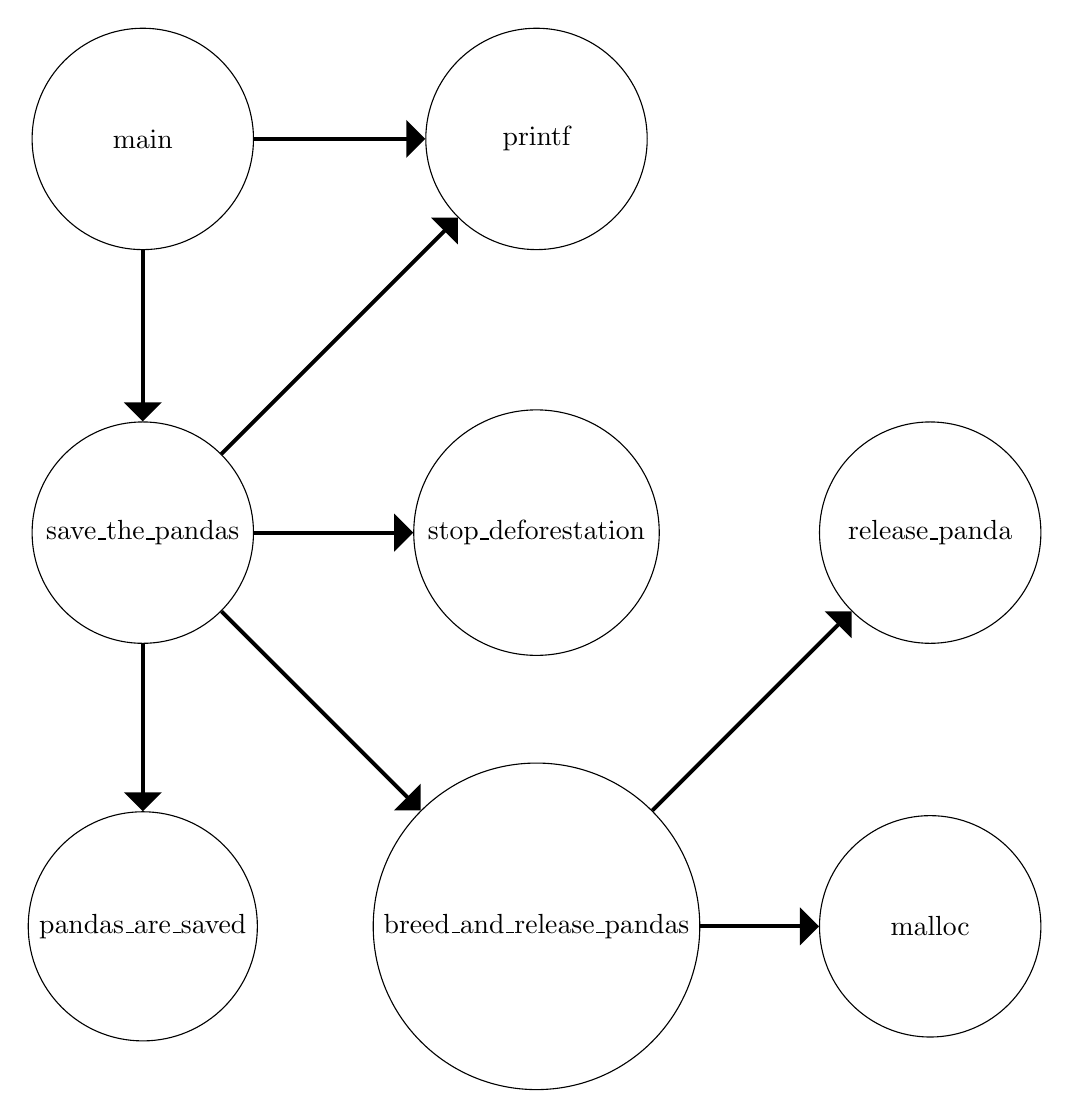
\begin{tikzpicture}[scale=1.0]
        \tikzset{vertex/.style = {shape=circle,draw,minimum size=8em}}
        \tikzset{edge/.style = {->,> = latex'}}
        % vertices
        \node[vertex] (main) at
            (0,0) {\lstinline{main}};
        \node[vertex] (savethepandas)
            at  (0,-5) {\lstinline{save_the_pandas}};
        \node[vertex] (stopdeforestation)
            at  (5,-5) {\lstinline{stop_deforestation}};
        \node[vertex] (breedandreleasepandas)
            at  (5,-10) {\lstinline{breed_and_release_pandas}};
        \node[vertex] (printf)
            at  (5,0) {\lstinline{printf}};
        \node[vertex] (pandasaresaved)
            at (0,-10) {\lstinline{pandas_are_saved}};
        \node[vertex] (releasepanda)
            at (10, -5) {\lstinline{release_panda}};
        \node[vertex] (malloc)
            at (10, -10) {\lstinline{malloc}};
        %edges
        \draw[edge, -triangle 90, line width=0.5mm] (main) to (savethepandas);
        \draw[edge, -triangle 90, line width=0.5mm] (main) to (printf);
        \draw[edge, -triangle 90, line width=0.5mm] (savethepandas) to (stopdeforestation);
        \draw[edge, -triangle 90, line width=0.5mm] (savethepandas) to (breedandreleasepandas);
        \draw[edge, -triangle 90, line width=0.5mm] (savethepandas) to (pandasaresaved);
        \draw[edge, -triangle 90, line width=0.5mm] (savethepandas) to (printf);
        \draw[edge, -triangle 90, line width=0.5mm] (breedandreleasepandas) to (releasepanda);
        \draw[edge, -triangle 90, line width=0.5mm] (breedandreleasepandas) to (malloc);
    \end{tikzpicture}
    \caption{Example Call Graph.  The source code associated with this call graph is shown in Figure~\ref{lst:pandasource}}
    \label{fig:pandacallgraph}
\end{figure}


As demonstrated by figure \ref{fig:pandacallgraph}, if there is a call from function $X$ to function $Y$ in the source code, there will be an edge pointing from node $X$ to node $Y$ in the associated call graph.  We can say that $main$ directly calls $printf$ and $save\_the\_pandas$ and that $save\_the\_pandas$ directly calls $pandas\_are\_saved$, $stop\_deforestation$, and $breed\_and\_release\_pandas$ because there is an edge in the graph that directly connects these functions.  We can also say that $main$ indirectly calls $stop\_deforestation$ because there is a path from $main$ to to $stop\_deforestation$.

Let us now imagine that there is some constraint whereby $save\_the\_pandas$ is not allowed to touch the heap.  Using existing tools, it would be possible to bar any function anywhere in the codebase from calling $malloc$ or to simply link to a nonstandard library without $malloc$ defined.  This solution is problematic, however, because now no entity in the entire codebase can call $malloc$.  What would be more useful is a system of marking functions that cannot call $malloc$ and having a tool check the call graph to make sure it does not happen.  




\chapter{Related work}\label{sec:related}

Static program analysis is a hot topic in Computer Science research.  The Association for Computing Machinery (ACM) publishes several journals, such as Proceedings of the ACM on Programming Languages (PACMPL), Transactions on Programming Languages and Systems (TOPLAS), and Transactions On Software Engineering and Methodology (TOSEM), which are focused (at least in part) on static verification and type systems.  It should come as no surprise that there is a large body of research that is related to this thesis.  This Chapter references a tiny fraction of this body of work.  Section \ref{sec:related:effectiveness} calls upon past research to assert unquestionably the positive impact that static analysis has on the software development process.  Section \ref{sec:related:aftermarket} explores a line of research dedicated to inserting supplemental specifications into existing programming languages in order to improve the static checkability of those languages.  Lastly, Section \ref{sec:related:libclang} pays respect to the LLVM project which has enabled so much of the research for this thesis.

\section{On the Effectiveness of Static Analysis}\label{sec:related:effectiveness}

Studies have long shown that static analysis is an essential tool for developing high-quality software.  The high speed and low cost of this type of verification make it an economical method for finding faults in program code~\cite{staticanal, static-anal-experience}.  

Industry has taken this observation to heart.  Many companies have their own internal tools dedicated to statically checking code changes with a goal of detecting common mistakes and stylistic issues.  The Mozilla project is a good example of this --- since the early 2000s, Mozilla has used a fairly robust suite of internal tools specifically crafted for Mozilla's mostly C++ codebase.  Using these tools, every Pull Request into Mozilla Firefox is parsed and checked against a set of hand-written rules to detect and report common issues~\cite{mozilla-pork-blog, moz-wiki-static-anal}.  Much of this tooling was dedicated to detecting memory issues.  Of course, without modifying the grammar of C++, there are limitations in what can be easily checked statically by these tools.  Only a small subset of the problem could be effectively detected.  

More recently, Mozilla developed and began using a language called Rust which was designed with certain static analysis characteristics in mind.  The Rust language implements an innovative type system meant to formally track the ownership of objects in memory.  ``Rust's type system and runtime guarantee the absence of data races, buffer overflows, stack overflows, and access to uninitialized or deallocated memory''~\cite{rust-is-dope}.  A common sentiment in the Rust-language community is that even though the ``Borrow Checker'' (the part of the type system that enforces memory safety) seems complicated at first, seasoned Rust users learn to depend on it to help them reason through complicated programs~\cite{rust-lang-spec}.  Rust demonstrates that making a type system more expressive and more restrictive can improve both the static checkability of a programming language and also the help the users of those languages.  

\section{Aftermarket Type Systems --- Supplementing an Existing Language}\label{sec:related:aftermarket}

The idea of introducing new forms of type checking into an existing language to increase safety is nothing new.  As early as 1994 tools such as LCLint have existed which allow the programmer to write down specifications about their code that are not necessarily supported by the original language standard.  The LCLint tool can take program source code as well as a file containing supplemental specifications and perform static analysis that is more thorough and informed than could possibly be achieved based on the language standard alone~\cite{lclint-og}. 

A useful attribute of these supplemental static analysis tools is that they scale incrementally --- the programmer can use these tools to whatever extent they find helpful and can increase or reduce the amount of information they pass on to these tools as they see fit.  Since these specifications are opt-in, adding new forms of specification to a tool like LCLint is a straightforward way to expand the scope of the tool without breaking backwards compatibility.  As an example, in 1996, Evans \textit{et al}. added a few variable type annotations to LCLint such as \lstinline{not-null}, \lstinline{possibly-null}, and \lstinline{null}.  When used by the programmer, these annotations allow LCLint to check for certain kinds of errors relating to nullness and memory allocation~\cite{lclint-memory}.  Such modifications require zero action by the users that choose not to use them; if a variable is not annotated then LCLint will not try to check that variable.  However, as the user adds more annotations, LCLint is able to check more variables.  The amount of feedback LCLint is able to provide scales up and down with the amount of annotations in the code.  

In general, variable annotations like \lstinline{not-null} and \lstinline{possibly-null} are very similar in use to the existing system of type qualifiers in the C family of languages.  A canonical example of a type qualifier would be the C \lstinline{const} qualifier; a variable marked \lstinline{const} may be set once at declaration but never updated again (ignoring unsafe casts).  Type qualifiers and annotations like \lstinline{const} and \lstinline{not-null} have two benefits:  First, they declare the intent behind the code so that other programmers reading the code have a better idea of how it works.  Second, they dictate what the programmer can and cannot do with an identifier so that the compiler or other static checking tool can detect accidental misuse.  However, their use is entirely optional --- the programmer can choose to treat an identifier as \lstinline{const} or \lstinline{not-null} without actually adding the annotation~\cite{theory-of-qual}.

``A Theory of Type Qualifiers'' develops this concept in depth and explores the theoretical and practical concerns involved with using type qualifiers in a language~\cite{theory-of-qual}.  One of the most relevant observations to the work in this paper is that every type qualifier introduces a form of subtyping.  For all types $T$ and any qualifier $q$, either $T \leq q T$ or $q T \leq T$ depending on $q$\footnote{This notation is equivalent to the subset notation (i.e., $T \subseteq q T$ or $q T \subseteq T$).  We choose to use the less than operator because it matches the notation used by Foster in ``A Theory of Type Qualifiers''.}.  Here we notate $T$ qualified by $q$ as $q T$ and we notate $X$ is a subtype of $Y$ as $X \leq Y$.  $X \leq Y$ should be interpreted to mean that $X$ can be safely used whenever $Y$ is expected.  For example $\lstinline{int} \leq \lstinline{const int}$ because in any statement containing a $\lstinline{const int}$, one could safely substitute an $int$ however the reverse is not true.  In the same vein, $\lstinline{not-null char*} \leq \lstinline{char*}$ because any statement referencing a $\lstinline{char*}$ could safely be given a $\lstinline{not-null char*}$ instead~\cite{theory-of-qual}.  In this paper we will apply this concept to the type qualifiers introduced by funqual in order to argue for the correctness of funqual.  

\section{libClang and the Explosion of C++ Tooling}\label{sec:related:libclang}

C++ is difficult to parse~\cite{cpp-sucks, libclang-survey, mozilla-pork, parse-cpp}.  Years of language additions, the need for backwards compatibility, and the existence of a text-based preprocessor\footnote{In theory, preprocessing could be delegated to another tool like gcc.  In practice this generally leads to loss of information --- most notably with \lstinline{#include} directives obfuscating the locations of symbols in source code.} means that the language grammar is large and complicated.  As a result, even the simplest static analysis tools require a huge amount of complexity to do basic parsing of source code.  Up until relatively recently, many C++ language tools settled on doing a partial parse of the language using approximations and heuristics~\cite{libclang-survey}.  This method can lead to artificial constraints on the language or to incorrect interpretations of the source.  

As a result of the LLVM Compiler Infrastructure Project, we now have an excellent set of tools for working with code.  The Clang compiler is a fully featured compiler from the LLVM project that supports a wealth of C-family language standards including C++17.  The LLVM project also provides libClang which exposes a convenient API to the parser and the AST used by the Clang compiler.  libClang enables developers to create their own tools that build on top of Clang's C++ parser.  This means that developers of static analysis tools only need to focus on maintaining their project's contributions rather than supporting an entire parser/AST toolsuite~\cite{libclang-survey}.  Funqual is built using libClang and so the work done in this paper was only possible thanks to the work done by the LLVM Compiler Infrastructure Project.  


\chapter{Validation}

This chapter examines some of the unique properties that a tool like funqual needs to respect in order to function properly as well as how those properties were tested both in the code and in practice.  

\section{Bridging the Divide between Translation Units}

The compilation of C++ code is driven by translation units.  Translation units are the files which are inputted into the C compiler to be translated into object files.  In general, translation units are singular $.c$ or $.cpp$ files where the preprocessor has already expanded all macros (including $#include$ substitutions).  During this process, many symbols are said to have $external linkage$ meaning that their type is specified in this translation unit but not their value or definition (this is the case with extern variables, function prototypes, and class forward declarations).  In these cases, examining the call tree of a single translation unit is not sufficient to enforcing global call-tree constraints because we would be able to see which internally linked functions call externally linked functions but not vise versa.  

To solve this problem we need to examine every translation unit in the source tree and build a call tree which represents the entire codebase.  In order to test this, we create several test cases where functions are defined in multiple translation units and where function a call tree constraint is violated between translation units.

\section{Dealing with Inheritance}\label{sec:val:inherit}





\nocite{*}
\bibliography{bibliography}

% Indents Appendix in Table of Contents
\makeatletter
\addtocontents{toc}{\let\protect\l@chapter\protect\l@section}
\makeatother

% Hack to make Appendices to appear in Table of Contents
\addtocontents{toc}{%
   \noindent APPENDICES
}
\begin{appendices}
\input{appendix-outline}
\end{appendices}

\end{document}
